\section{Results} \label{sec:Results}

%%%%%%%%%%%%%%%%%%%%%%%%%%%%%%%%%%%%%%%%%%%%%%%%%%%%%%%%%%%%%%%%%%%%%%%%%%%  
%% JUST THE OBJECTIVE FACTS, no interpretation or discussion
%%
%% what exactly did you do
%%  
%% what were the inputs/outputs/parameters
%%  
%% what computer hardware
%%  
%% what software
%%  
%% what were the results
%%  
%% tables/figures/plots
%%  
%% error analysis
%%%%%%%%%%%%%%%%%%%%%%%%%%%%%%%%%%%%%%%%%%%%%%%%%%%%%%%%%%%%%%%%%%%%%%%%%%%  

Here we shall present the results that we acquired from our experiments. We will
describe our generic testbed, so should the reader wish to follow along in
real time they may have the option of doing so. After this, the performance 
of each brain will be evaluated individually. Finally we will compare the models
to each other.

\subsection{Testbed}
All of our experiments were performed within the Flatworld II v.1.0 
environment. Our code was written in Python 2.6, and interfaced with 
Flatworld's C-based API via a shim (see section \ref{sec:Ack}). All of our
runs were done on a Lenovo ThinkPad W510 with an Intel i7 quad core processor
and 16GB of DDR3 RAM. Windows 7 Pro 64bit is the machine's native platform,
but we ran our tests inside a virtual machine using VMware 8.04. The virtual
machine was configured with Ubuntu 10.04 32bit, 1GB of RAM and a single 2GHz
processor. We used Matplotlib 1.2 for our data figures.


\subsection{Brain 0}
We start our data presentation with Brain 0 (a very good place to start).
It should come as no surprise that brain 0's lifespan is 2000 time steps. 
The agent makes no moves, and makes no attempts to eat anything. 
Figure \ref{fig:brain0energy} shows an agent's average energy depletion over 
time based upon 153 runs. When the agent is idle, the energy decreases 
linearly. The bar has been set, as they say.

\begin{figure}
\begin{center}
  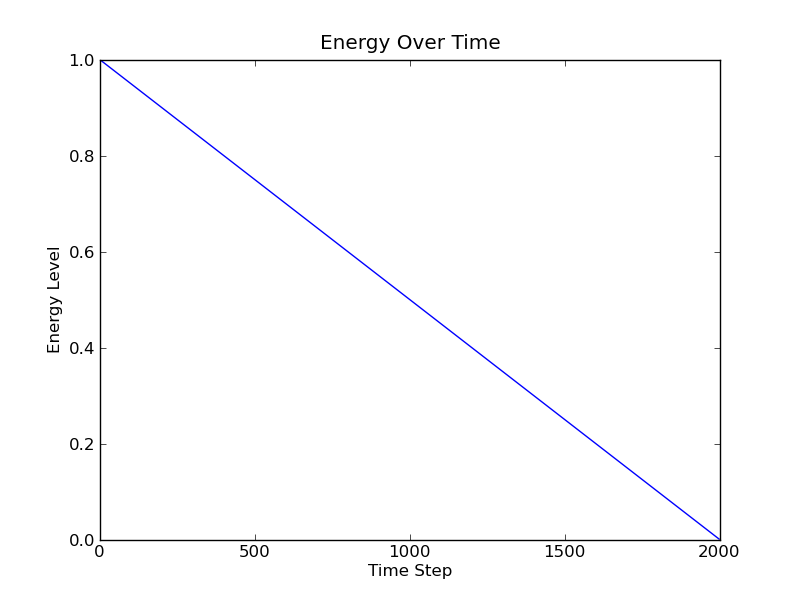
\includegraphics[scale=.65]{plots/brain0energy.png}
  \caption{Agent's energy level over time ($\sigma = 0$)}
  \label{fig:brain0energy}
\end{center}
\end{figure}

Figure \ref{fig:brain0his} is a histogram which also confirms the average 
lifespan of our agents to be exactly 2000 time steps.

\begin{figure}
\begin{center}
  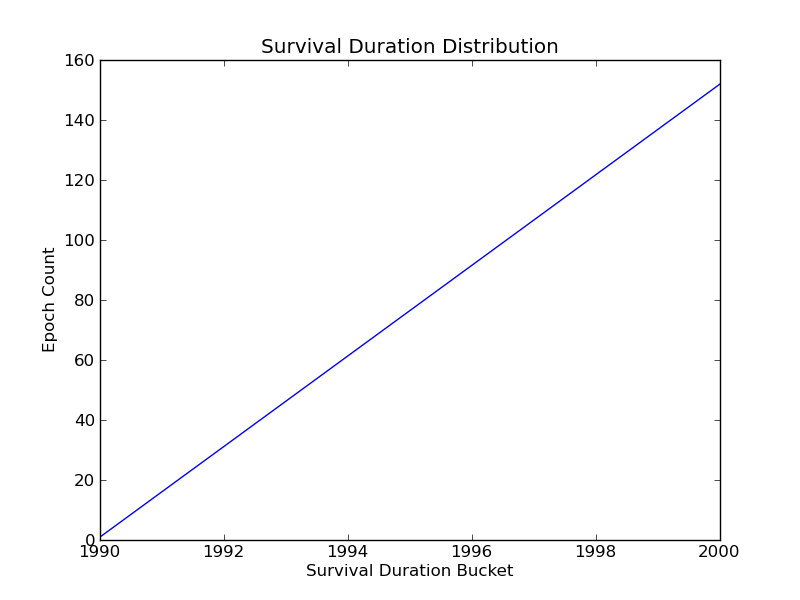
\includegraphics[scale=.65]{plots/brain0hist.png}
  \caption{Agent lifetimes for Brain 0 ($\sigma = 0$)\\
  (Note: this is Matplotlib's attempt to plot a linear distribution of
  a single data point)}
  \label{fig:brain0his}
\end{center}
\end{figure}


\subsection{Brain 1}
It may be a surprise that Brain 1's performance worse than that of Brain 0. 
This is due to the fact that not only is
it relying on food to be directly in its path, but it also is expending 
\emph{more} energy from the act of moving. Figure \ref{fig:brain1velo} shows
that increasing the agent's velocity will cause its energy to decrease
exponentially.

\begin{figure}
\begin{center}
  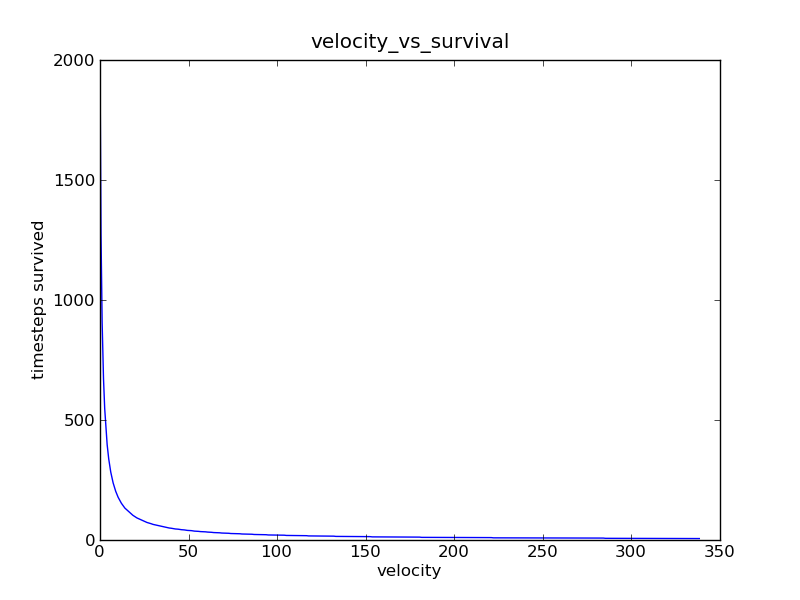
\includegraphics[scale=.65]{plots/brain1velo.png}
  \caption{An agent's lifespan as a function of velocity}
  \label{fig:brain1velo}
\end{center}
\end{figure}

\begin{figure}
\begin{center}
  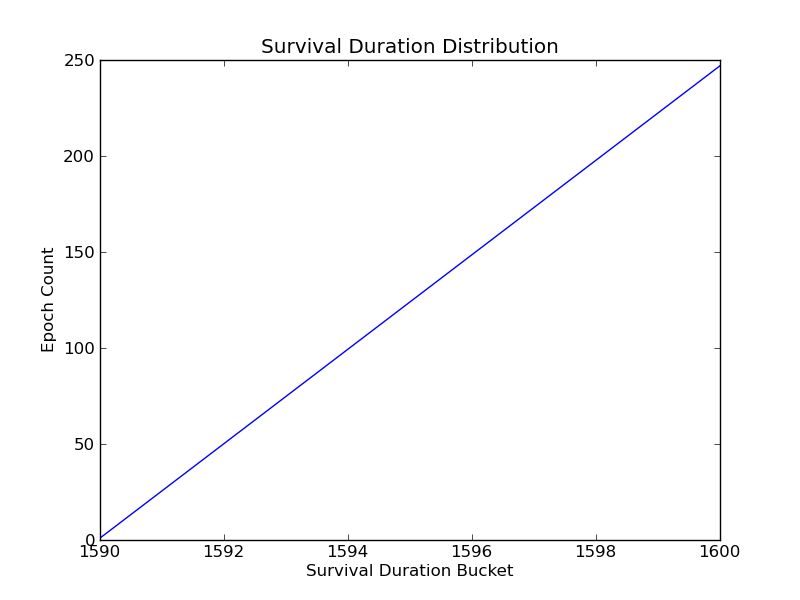
\includegraphics[scale=.65]{plots/brain1hist.png}
  \caption{Agent lifetimes for Brain 1 ($\sigma = 0.11$)\\
  (Again... Matplotlib)}
  \label{fig:brain1his}
\end{center}
\end{figure}

The histogram in figure \ref{fig:brain1his} illustrates agents' lifetimes based
off of a constant velocity value of 0.25. There was very, very little change
in lifetime from run to run. The average survival time of 248 runs was 
1600.00.

\subsection{Brain 2}
Brain 2 performed less effectively than Brain 1, despite the addition of the
eyelet neuron. The average lifespan for agents endowed with Brain 2 was 
1557.85.

\begin{figure}
\begin{center}
  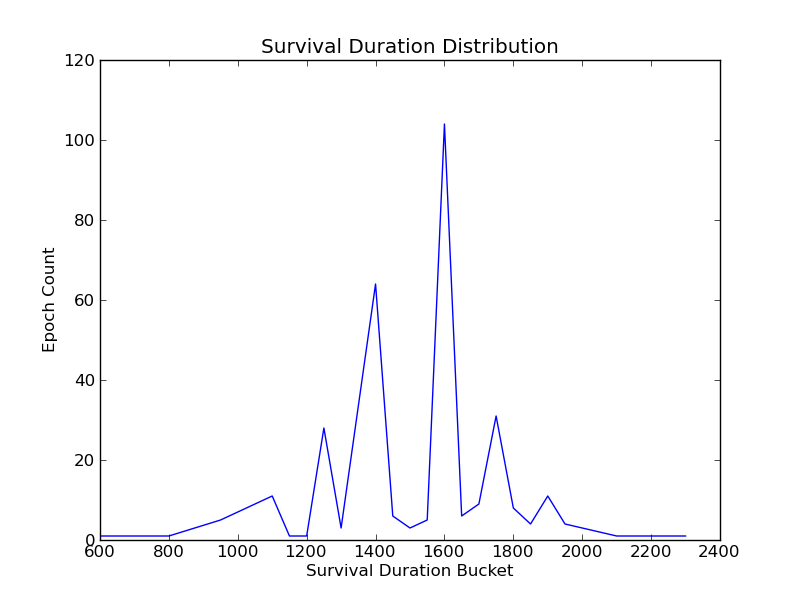
\includegraphics[scale=.65]{plots/brain2hist.png}
  \caption{Agent lifetimes for Brain 2 ($\sigma = 227.88$)}
  \label{fig:brain2his}
\end{center}
\end{figure}

\subsection{Brain 3}

\begin{figure}
\begin{center}
  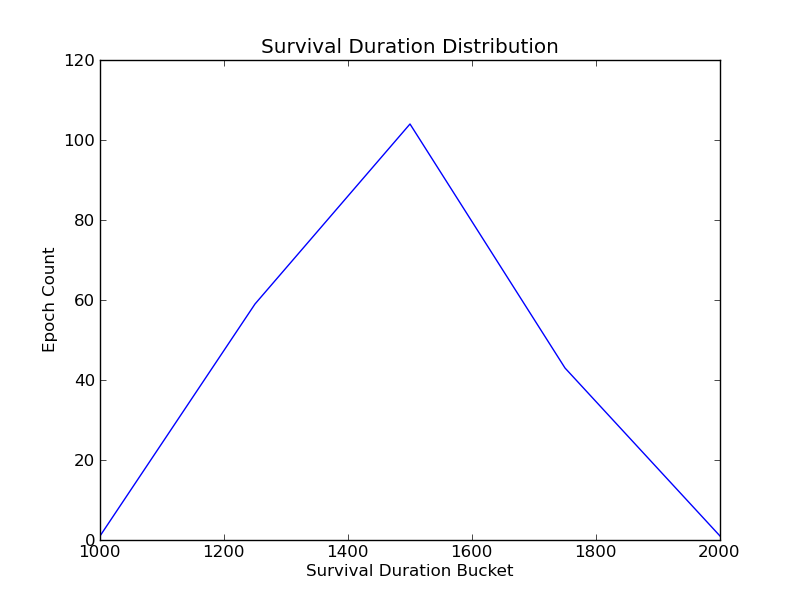
\includegraphics[scale=.65]{plots/brain3hist.png}
  \caption{Agent lifetimes for Brain 3 ($\sigma = 153.55$)}
  \label{fig:brain3his}
\end{center}
\end{figure}

Brain 3, which introduced the sigmoid neuron, also performed more poorly
than Brain 0, with an average lifespan of 1581.63. The standard deviation
improved from Brain 2, though.

\begin{figure}
\begin{center}
  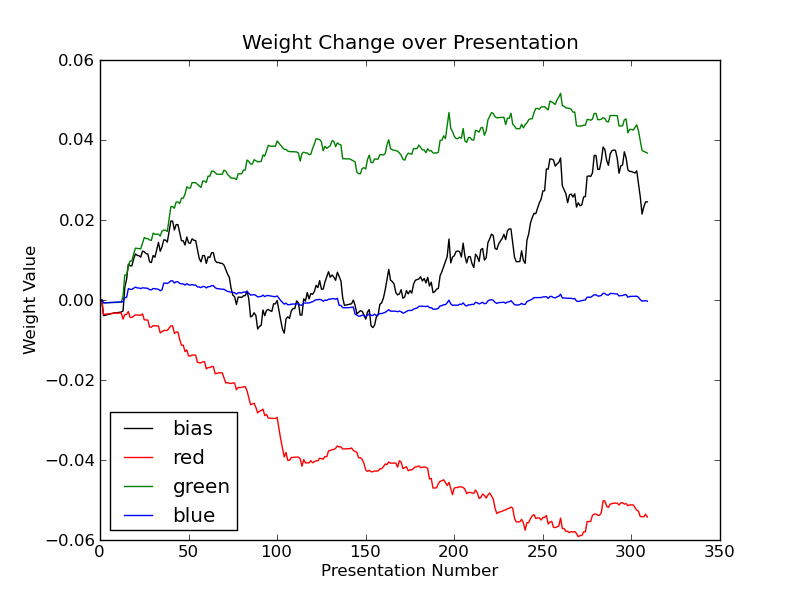
\includegraphics[scale=.65]{plots/weights.png}
  \caption{Weight change for sigmoid neuron}
  \label{fig:brain3wghts}
\end{center}
\end{figure}

Also, via figure \ref{fig:brain3wghts}, you can see that the sigmoid neuron 
was behaving properly; weights were
adjusted after viewing each object using the following formula\cite{Haykin}:

\begin{equation}
  w_i(n+1) = w_i + \eta e(n) \varphi'(n) x_i(n)
\end{equation}

This neuron will produce a positive value if it thinks it's seeing a food 
object, a negative value if it thinks the object is poisonous, and a near-zero
value if it thinks it's neutral.

At this point we should mention that, after we had satisfactory 
convergence, we decided to turn off learning for future sigmoid neuron(s). The 
trial runs we had for Brain 3 proved that our color
classifier neuron was indeed doing its job.


\subsection{Brain 4}

\begin{figure}
\begin{center}
  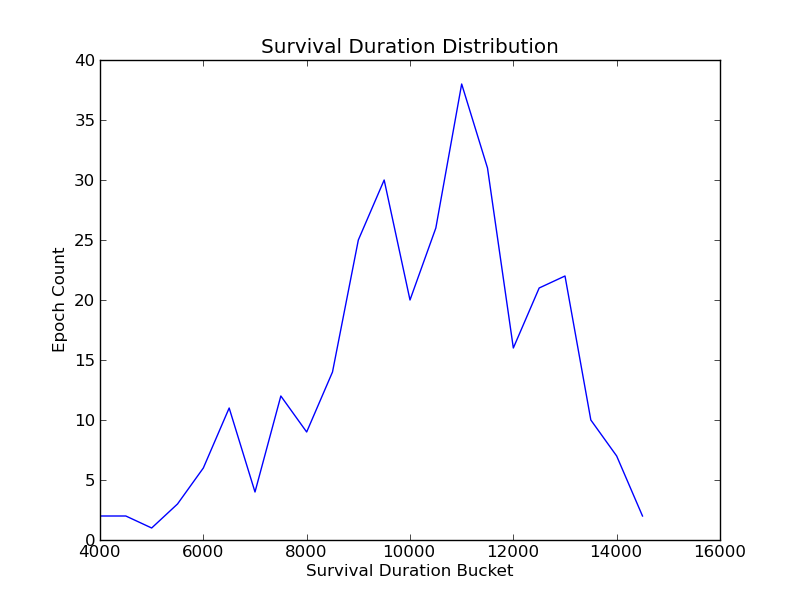
\includegraphics[scale=.65]{plots/brain4hist.png}
  \caption{Agent lifetimes for Brain 4 ($\sigma = 2154.90$)}
  \label{fig:brain4his}
\end{center}
\end{figure}

Agents sporting Brain 4 lived to ripe ages that had not been seen in previous
models (fig. \ref{fig:brain4his}); the average agent has a lifespan of about
12480. This is also the first brain 
to implement a WTA network for the visual cortex and allow for rotation.


\subsection{Brain 5}

\begin{figure}
\begin{center}
  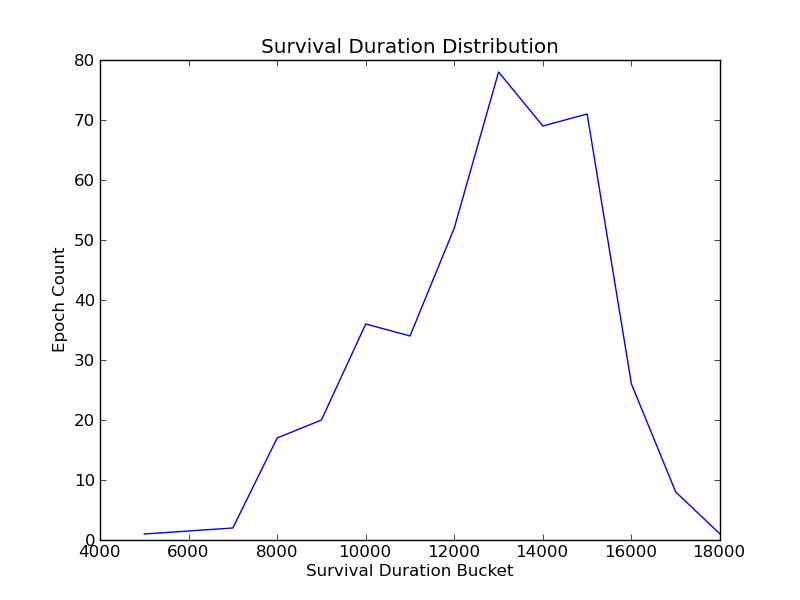
\includegraphics[scale=.65]{plots/brain5hist.png}
  \caption{Agent lifetimes for Brain 5 ($\sigma = 2289.75$)}
  \label{fig:brain5his}
\end{center}
\end{figure}

Brain 5 is the combination of Brains 3 and 4. The average lifetime for 446
agents with Brain 5 was 13238; despite the combination, that netted just 
slightly less than a 6\% improvement over Brain 4's average lifetime. 


\subsection{Brain 6}
\begin{figure}
\begin{center}
  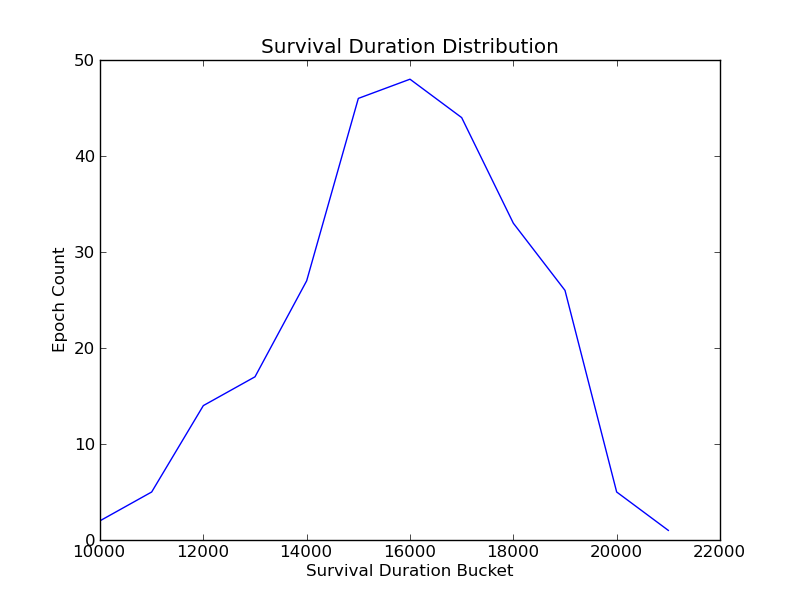
\includegraphics[scale=.65]{plots/brain6hist.png}
  \caption{Agent lifetimes for Brain 6 ($\sigma = 2143.33$)}
  \label{fig:brain6his}
\end{center}
\end{figure}

Agents equipped with Brain 6, who consider object color before causing the 
agent to eat, saw further improvement (fig. \ref{fig:brain6his}). The average 
time-to-death of agents was 16374.08. The standard deviation also decreased.


\subsection{Brain 7}
\begin{figure}
\begin{center}
  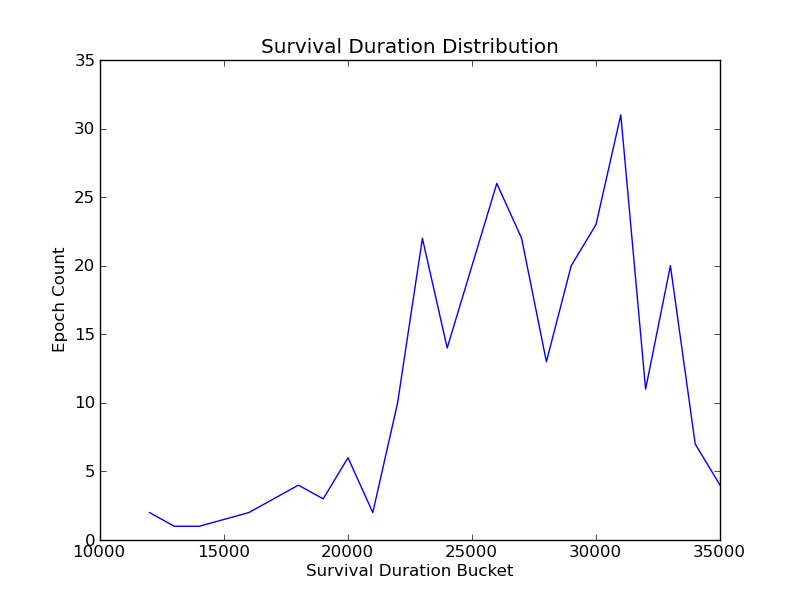
\includegraphics[scale=.65]{plots/brain7hist.png}
  \caption{Agent lifetimes for Brain 7 ($\sigma = 4523.73$)}
  \label{fig:brain7his}
\end{center}
\end{figure}

Brain 7 saw another massive jump in vitality 
(fig. \ref{fig:brain7his}). An average lifetime of 27623.54 is an improvement
of approximately 40\% over Brain 6. Note, too, that there is a large increase 
in the standard deviation of those lifetimes.


\subsection{Brain Comparison}
\begin{figure}
\begin{center}
  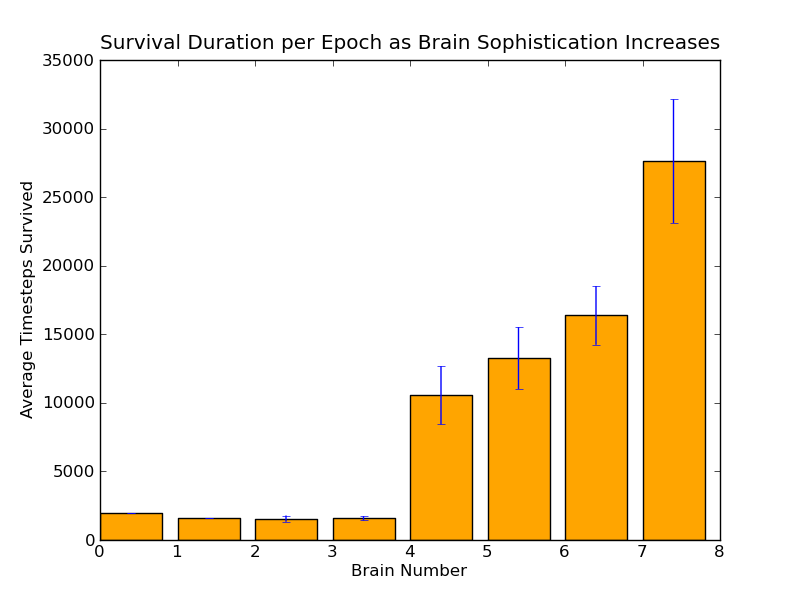
\includegraphics[scale=.65]{plots/survive.png}
  \caption{Agent lifetimes across all 8 brains}
  \label{fig:survive}
\end{center}
\end{figure}

Figure \ref{fig:survive} shows a side-by-side comparison of an agent's 
projected lifespan given its brain model.
